% This is LLNCS.DEM the demonstration file of
% the LaTeX macro package from Springer-Verlag
% for Lecture Notes in Computer Science,
% version 2.4 for LaTeX2e as of 16. April 2010
%
\documentclass{llncs}

\usepackage[utf8]{inputenc} 
\usepackage{cite}
\usepackage{listings}
\usepackage[usenames,dvipsnames]{color}
\usepackage{hyperref}
\usepackage{scrpage2}
\usepackage{graphicx}
\automark[subsection]{section}% section auf linker, subsection auf rechter Seite
\pagestyle{scrheadings}

\definecolor{orange}{RGB}{255, 235, 235}
\lstset{numbers=left, numberstyle=\tiny, stepnumber=1, numbersep=5pt, basicstyle=\small, stringstyle=\ttfamily, showstringspaces=false, emph={S, NP, VP}, emphstyle=\underbar, xleftmargin=2pt, xrightmargin=2pt}

% Bullets for list items
\renewcommand{\labelitemi}{$\bullet$}

%
%\usepackage{makeidx}  % allows for indexgeneration
%
\begin{document}
%
\frontmatter          % for the preliminaries
%
%\pagestyle{headings}  % switches on printing of running heads
%
\mainmatter              % start of the contributions
%
\title{Analysing differences in tree-structured data
by Visual Analytics}
%\subtitle{Grammatikentwicklung in XLE/LFG}
%
%\titlerunning{Quenya - Grammatikentwicklung}  % abbreviated title (for running head)
%                                     also used for the TOC unless
%                                     \toctitle is used
%
\author{Johannes Lichtenberger}
%
\institute{University of Konstanz, Germany\\
\email{\href{mailto:Johannes.Lichtenberger@uni-konstanz.de}{Johannes.Lichtenberger@uni-konstanz.de}}}

\maketitle              % typeset the title of the contribution

\begin{abstract}
Current state of the art line-based diffing algorithms and visualizations thereof aren't tree aware. Furthermore almost all recent tree-aware diff-visualizations aren't able to explicitly highlight inserted-, deleted-, replaced- as well as updated-nodes. Thus, we propose different solutions based on a SunburstView.
\end{abstract}
%
\section{Motivation}
Current state of the art line-based diffing algorithms and visualizations on tree-structured data aren't sufficient. XML, which is a tree-structured meta markup-language, adds further constraints.

In a nutshell line based LLCS algorithms such as \texttt{GNU-diff}, \texttt{(g)vimdiff} etc.pp. are not tree-aware and have no knowledge about XML semantics which results in

\begin{itemize}
\item Mismatches of element nodes with different \texttt{QNames}.
\item Matches across node-boundaries.
\item \texttt{Attribute}- and \texttt{namespace}-order changes are considered as a change.
\item Whitespace between attributes or namespaces are considered as a change.
\end{itemize}

Figure \ref{fig:gvimdiff} illustrates some of these drawbacks on two revisions of a simple XML-document. For larger XML instances it is mandatory to scroll, thus additionally losing the overview about the whole file is another drawback.

\begin{figure}[htb]
\center{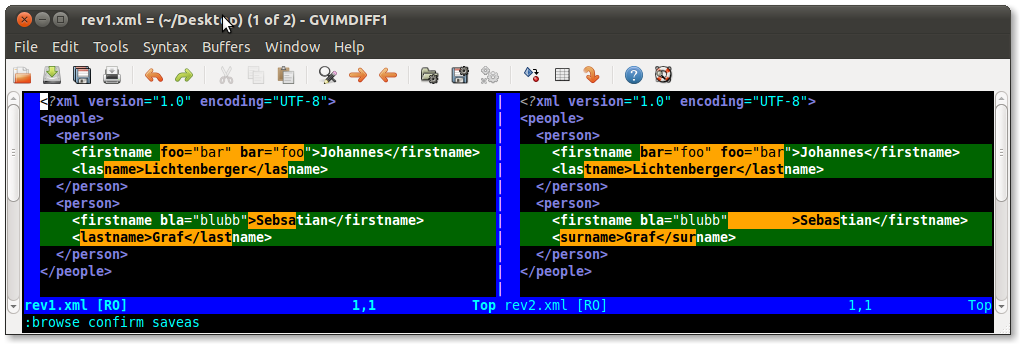
\includegraphics[width=\textwidth]
{../images/gvimdiff.png}}
\caption{\label{fig:gvimdiff} Comparsion of two revisions of a simple XML-document with gvimdiff.}
\end{figure}

\subsection{Application domains}

Motivating examples are manyfold. To meantion just a few of them:

\begin{itemize}
\item Even though companies and the relationship among employees in general form a directed acyclic graph (DAG) most of them are organized in a hierarichal tree-structure \footnote{also referred to as a connected acyclic graph (CAG)} which evolves over time. Appropriate representations of the changes enables to track the career of certain persons or might reveal how sub-organizations are evolving very well while others might not due to the success or failure of products.
\item The hierarichal structure of filesystems and the recently upcoming abilities to store Snapshots, which is based on the COW (copy-on-write) implementation of recent filesystems like BtrFS and ZFS. Users might want to quickly determine when and where directories/files have been moved, when they have been deleted or created and so forth. An example application which recently reached end users through Apples' OS X is TimeMachine. Furthermore permission rights of files can be tracked through time, which might be of great value to security engineers.
\item Humans which are interested in detailed changes of several versions of some products and compare their attributes and features. This analysis might even reveal how companies prioritise the development and enhancement of certain features.
\item Tracking changes in software development based on a low level Abstract Syntax Tree (AST) comparsion. This might reveal code splits, merges, deletions and inserts. At a greater scale constant unmodified code can be tracked through several revisions revealing stable code in contrast to new features. The latter usually is subject to many changes.
\item Biologists have to understand structural differences of phylogenetic/evolutionary trees which in general can be very large. An efficient comparsion algorithm is needed as well as some kind of visual interface to asses biologists in locating and exploring tree differences.
\end{itemize} 

\section{Proposed visualizations}
\subsection{SunburstView}
In contrast our first proposed visualization (Figure \ref{fig:treetank-gui}) used on a XML-document with about 800 nodes displays detailed differences of the tree data itself and is aware of XML semantics. Two revisions of a Treetank-\texttt{resource} can be compared. The \emph{SunburstItem}s, which represent nodes and are located between the inner ring and the root node (the center) contain nodes which haven't been changed at all. Changed nodes are projected to the outer ring. The colors denote different operations in which a node has been changed. A legend is available in the bottom right corner.

It is roughly based on \cite{generative-gestaltung}, but now adheres to the well known MVC-architecture, whereas the model(s) in conjunction with a special \texttt{SunburstDescendantAxis} interact with Treetank. Furthermore besides the addition of the whole diff-view, our visualization in contrast uses an offscreen-buffer for all \texttt{SunburstItem} instances and was basically rewritten from scratch to adhere to good object oriented practices and design patterns. Left-over are some drawing mechanisms (which are now implemented based on the strategy pattern) such as the drawing of the \emph{SunburstItem}s and the connection splines to emphasize the \texttt{parent/child}-relationship.

\begin{figure}[htb]
\center{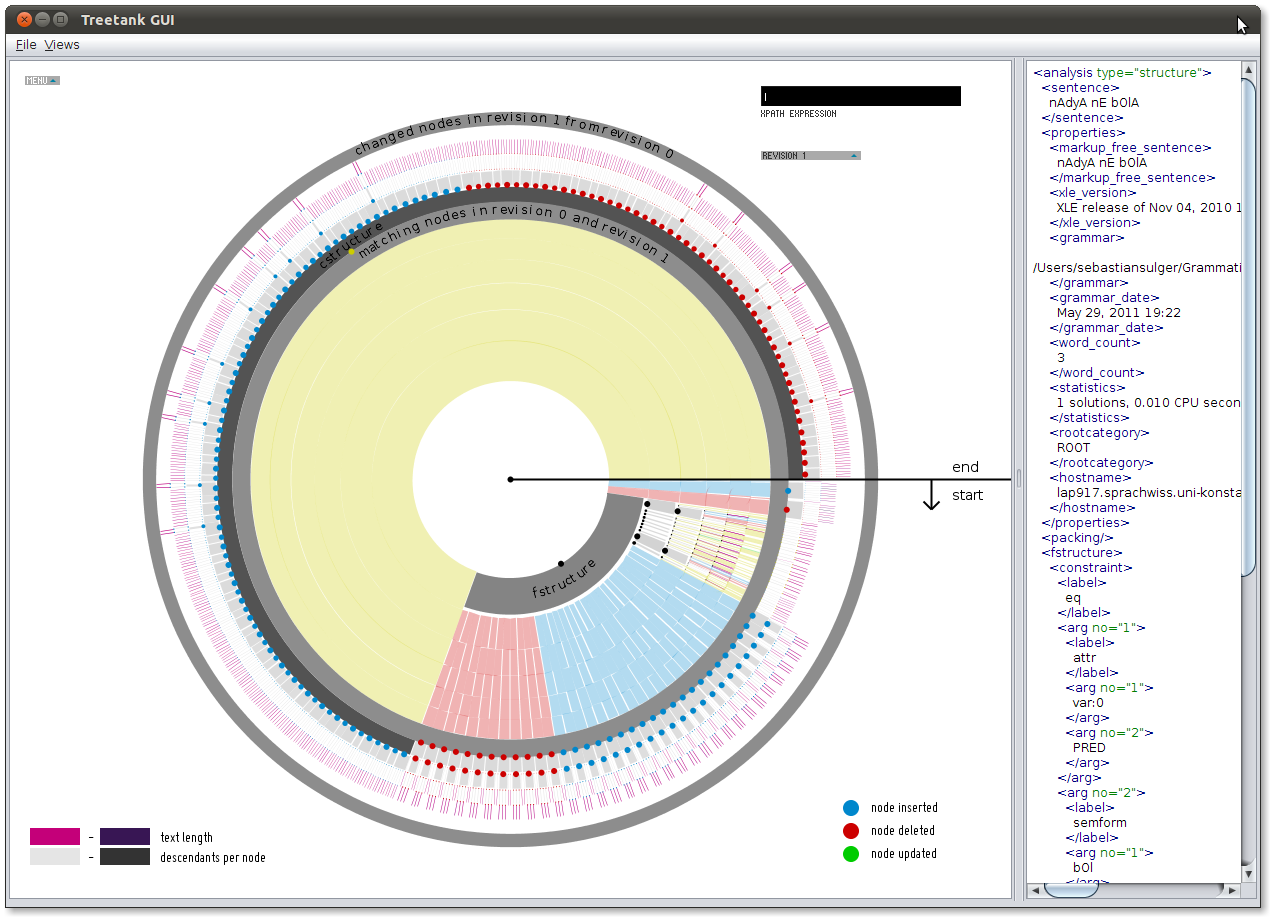
\includegraphics[width=\textwidth]
{../images/treetank-gui.png}}
\caption{\label{fig:treetank-gui} Comparsion of two revisions of an XML-document with approximately 800 nodes.}
\end{figure}

Currently our visualization is able to differentiate between the following \texttt{edit}-operations.

\begin{itemize}
\item \texttt{insertion} of a node.
\item \texttt{deletion} of a node.
\item \texttt{update} of a node, which is updating the \texttt{QName} in case of an element-node or the value in case of a text-node.
\item \texttt{replace} of a node with another node.
\end{itemize}

\subsection{SunburstView challenges}
Challenges while implementing the \emph{SunburstView} were manyfold:

\begin{itemize}
\item Items require a \texttt{start-angle}, an \texttt{extension} or \texttt{end-angle}, \texttt{descendant-or-\\self-count}, \texttt{modification-count} and the kind of change (\texttt{inserted}, \texttt{deleted}, \texttt{updated} or \texttt{replaced}). The \texttt{modification-count} denotes how many modified nodes exist in the subtree rooted at the current node.
\item Agglomeration of two revisions into one tree-representation.
\item Pruning of the tree to allow the visualization to scale for even the largest XML instances.
\item Provide a global enlargement of subtrees with many changed nodes to further help tracking differences which also shrinks unchanged subtrees.
\item Computation of the maximum level in the tree of unchanged nodes.
\item Computation of the \texttt{descendant-or-self-count} per node in the new revision including deleted nodes.
\item Integration of views based on processing.org\cite{processing.org} which can be used just like any other Java library in a Swing-GUI (but problems arise due to heavyweight vs. lightweight components).
\item Providing labels if items are big enough.
\item Write all \texttt{SunburstItem}s into an offscreen buffer.
\item Improved mouseover-effect to display further details about currently hovered nodes and to determine at which position the text has to be plotted (right or left to the cursor, dependent on the space left to display the information).
\item Integration of zooming and a fisheye-transformation.
\item Three normalizations are available for the \texttt{SunburstItem} color which currently denotes either how many \texttt{descendant-or-self} nodes follow in the subtree of the node, or the String-length of text node values.
\end{itemize}

Most of these challenges culminated in a \texttt{SunburstModel} and a specialized \texttt{SunburstDescendantAxis} which is used to create \texttt{SunburstItem}s, the segments in the \emph{SunburstView} which represent the nodes in the tree. The agglomeration of two revisions into one tree requires the iteration over the newer of both revisions but to add deleted nodes at the right positions\footnote{iteration over the old revision but to add inserted nodes would have been possible as well}. Thus the Treetank \texttt{read}-transaction has to switch to the old revision whenever a deleted node is encountered and to switch back if no further deleted nodes follow which is illustrated in figure (\ref{fig:tree-axis}). Input to the \texttt{SunburstDescendantAxis} besides a \texttt{read-transaction} on the new revision is a list of diffs. Each element incorporates the kind of diff, the depth of the node in the old revision and the node in the new revision and the two nodeKeys of the nodes which have been compared. Each time \texttt{hasNext()} is called the first element of the list is removed.

\begin{figure}[htb]
\center{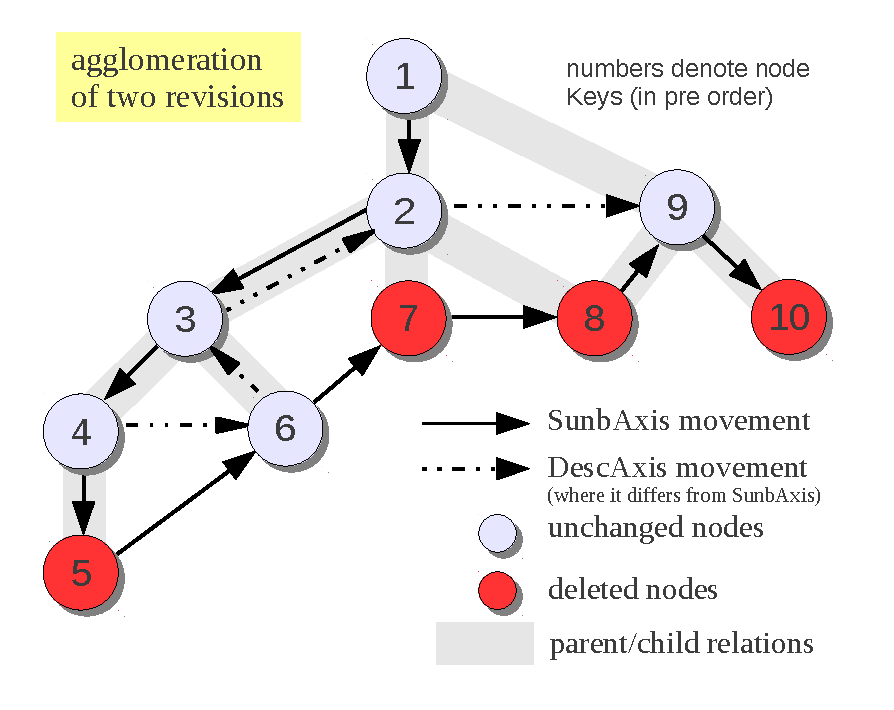
\includegraphics[width=0.6\textwidth]
{../images/tree-axis.pdf}}
\caption{\label{fig:tree-axis} Illustrates some challenges while developing the SunburstDescendantAxis which agglomerates two revisions into one tree.}
\end{figure}

One of the core challenges is to adjust the stacks for the \texttt{start-angle}, \texttt{extension}, \texttt{descendant-or-self-count} and the \texttt{modification-count} of each \texttt{SunburstItem} appropriately which is closely related to the challenge of fusing both trees together. If the transaction is located at node 4 it still has to push values onto the different stacks and remember this step. The \texttt{next-NodeKey} which would be usually 6 in the \texttt{DescendantAxis} is saved in a temporal variable to move to whenever no further deleted nodes are encountered\footnote{in the running example based on figure \ref{fig:tree-axis} after node 5}. Furthermore the next call to the iterator method \texttt{hasNext()} must change the current transaction which is a \texttt{read-transaction} on the new revision to a \texttt{read-transaction} on the old revision and modify member variables such as the \texttt{start-angle}, \texttt{extension}, and so on according to the previous step before the next \texttt{SunburstItem} is added. Located at node 6 the current active transaction must only call \texttt{pop()} once from all stacks which is actually one of the first things done the next time \texttt{hasNext()} is called. If an unchanged node would follow after node 6 (node 9 without considering deleted nodes) the stacks would be immediately adapted, e.g. \texttt{pop()} would have been called two times from all stacks since the next node (node 9) is located two levels above node 6. Another case occurs at node 9. If the new revision has no further nodes the diff-list has to be examined if deleted nodes are left.

Furthermore to get the maximum level for the nodes which haven't changed at all and to draw the ring at $maxLevel+1$ the algorithm iterates over the old revision but skips nodes with higher levels, which are actually deleted in the new revision.

\subsection{TextView}
The TextView is synchronized with the SunburstView (and the SmallMultiplesView) and provides pretty printed serialized XML as well as syntax highlighting and is scalable due to the fact, that initially only the viewport and some extra value is filled. Scrolling down adds more text depending on the scrollbar value change. Before a \texttt{StAXSerializer} which can be used for many other purposes has been developed.

\subsection{SmallMultiplesView}
\emph{SmallMultiples} divide the screen space into regions whereas each region displays a \emph{SunburstView} with different parameters to enable the analysis of the evolution of a tree.
Currently three variants of a \emph{SmallMultiplesView} are available. 

\begin{itemize}
\item An incremental view illustrating differences between successive revisions e.g. the differences between revision 0 and 1 illustrated in one SunburstView, the differences between revision 1 and 2 in another side by side and so on and so forth.
\item A differential view illustrating differences between the first and each successive revision. Assuming revision 0 is loaded and the \texttt{resource} has 10 revisions the comparsion of revision 0 and 1, 0 and 2, 0 and 3 and revision 0 and 3 are displayed through succesive \emph{SunburstView}s). Therefore at most four regions with a SunburstView are available just like in the other variants. However this is only a parameter which can easily be changed to 6 or 8 or another even value such that the screen space of larger monitors can effectively be utilized.
\item A hybrid view which displays the whole tree after the last revision (which is shown on screen) with every change made in the revisions in between. Then any changes which didn't occur in each successive incremental SunburstView are blackened.
\end{itemize}

Figure \ref{fig:treetank-gui-smallmultiples} depicts the last hybrid variant.

\begin{figure}[htb]
\center{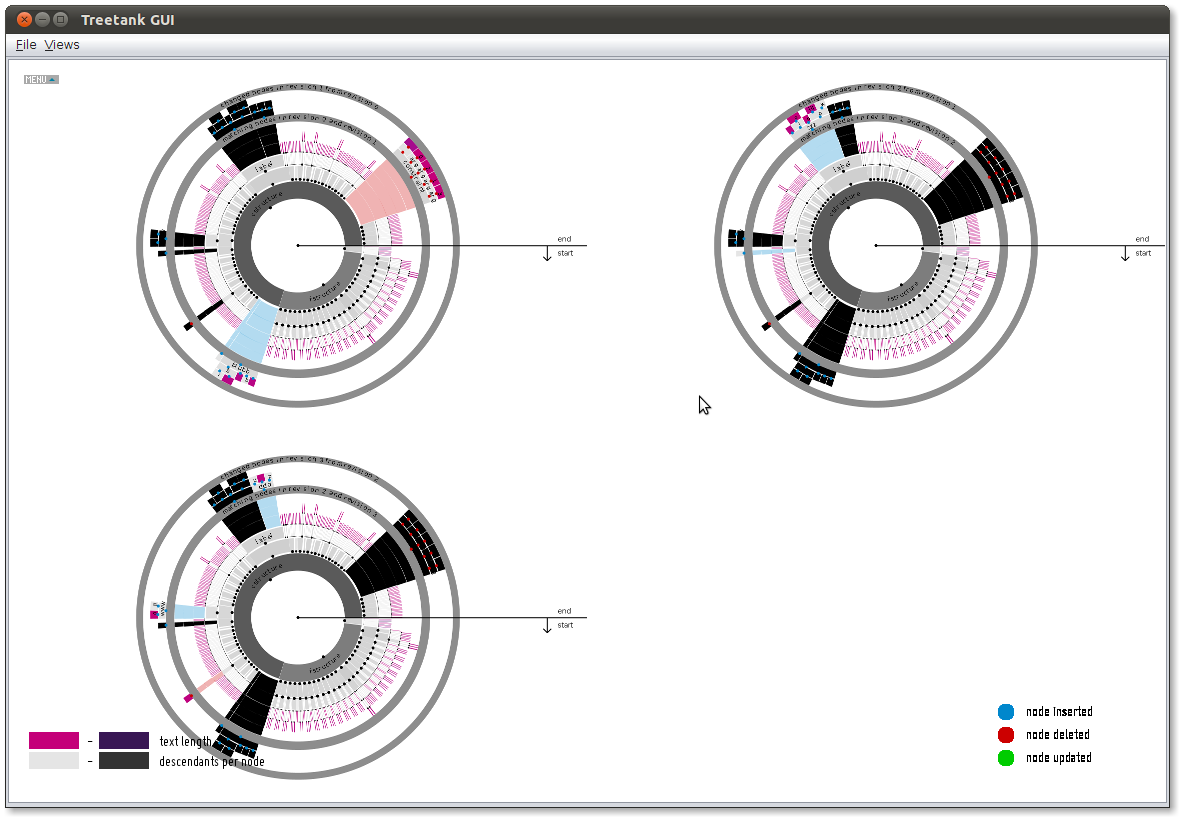
\includegraphics[width=\textwidth]
{../images/treetank-gui-smallmultiples.png}}
\caption{\label{fig:treetank-gui-smallmultiples} Comparsion of four successive revisions of an XML-document based on the hybrid variant.}
\end{figure}

\subsection{SmallMultiplesView challenges}
First of all further abstractions have been made to adhere to good software practices. A few of the challenges are:

\begin{itemize}
\item Since all (public) methods in every model\footnote{one component of the MVC architecture} are multithreaded the notification of observers (the GUI) about state changes have to be synchronized.
\item Multithreading also requires sorting of offscreen buffers such that the SmallMultiples are sorted from left to right to bottom.
\item In the hybrid view changes which haven't occured in an incremental diff between two successive revisions have to be blackened, respectively.
\end{itemize}

The third challenge is particular interesting. It involves the computation of differences between the first and last revision which can be displayed on screen (usually revision 0 to 4 with four different regions and incremental change views, the \emph{SunburstView}s). Next the \texttt{SunburstItem}s created during the incremental diff as well the comparsion between the first and last revision have to be sorted according to the \texttt{NodeKey} which is unique for each node. Then initially all nodes are blackened meaning their status is set to \texttt{BlackState.YES}. Thereafter a search is made to get the intersection of nodes. If nodes are equal according to the \texttt{java.lang.Object} method \texttt{boolean equal(Object paramItem)} nodes are colored ordinary, which means their greyout status is set to \texttt{BlackState.NO}. All nodes which are still in the status \texttt{BlackState.YES} are drawn in black.

\section{Tree-to-Tree Differences}
To compute the differences between two revisions initially two kinds of algorithms have to be distinguished, namely ID-less- and ID-based-algorithms. Figure \ref{fig:importdata} points out how these two kinds of algorithms are used in our approach. An ID-based algorithm has been developed and is used to compare revisions of a \emph{resource} in Treetank since each node has a unique \texttt{NodeKey} which identifies this node through time/all revisions even after updates. To speed up the algorithm, it optionally uses postorder-hashes which are per default generated during the shredding of an XML-document. If the hashes and the nodeKeys of both nodes match the whole subtree can be considered to be equal and therefore skipped. Thus the \texttt{read}-transactions move to the following nodes in both revisions. Yet this feature can't be used for the diff-view since each individual node has to be set to an explicit \texttt{diff}-state and the axis which has been developed needs to know the explicit diff-state for each node.

\begin{figure}[htb]
\center{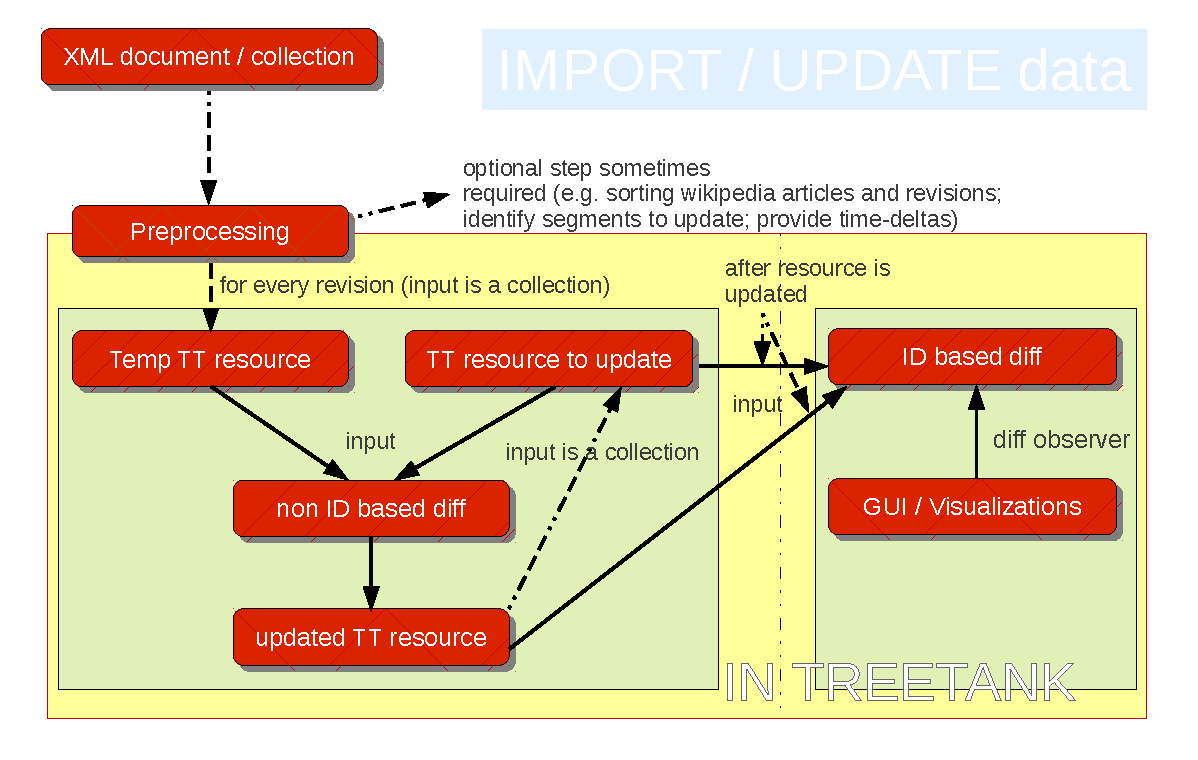
\includegraphics[width=\textwidth]
{../images/importdata.pdf}}
\caption{\label{fig:importdata} Illustrates when and how ID-less and ID-based diff-algorithms are used.}
\end{figure}

To import XML documents in Treetank in the first place the data sometimes has to be preprocessed. The following steps were necessary for the preprocessing of the Wikipedia dump with revision history of each article:

\begin{itemize}
\item Replace WikiText markup with well formed XML.
\item Sorting of articles and revisions based on timestamps with the MapReduce Framework of Apache Hadoop\cite{hadoop}.
\item Import based on different time-intervals.
\end{itemize}

An ID-less algorithm has to be used, which is usually slower due to the initial matching between nodes. Heuristics have to be used to speed up the matching algorithm since it's CPU time complexity to find "optimal" matches is at least $O(n^2)$ and above. Optimal matches are based on a cost model, which incorporates edit script costs. An edit script is a sequence of edit operations (usually insert, delete, update and move). Each edit operation is assigned a cost, which might be unit cost. An optimal matching between nodes yields a minimum edit script, which is an edit script whereas no other edit script exists with less overall cost, the sum of edit operation costs. During this initial phase of an algorithm nodes which are approximately equal also have to be matched which is illustrated in figure \ref{fig:matching}. Node 20 has been inserted but nontheless nodes 3 and 14 should match. Most of the algorithms use a \emph{Longest Common Subsequence} (LCSS) algorithm to match leaf nodes and sometimes also match inner nodes.

\begin{figure}[htb]
\center{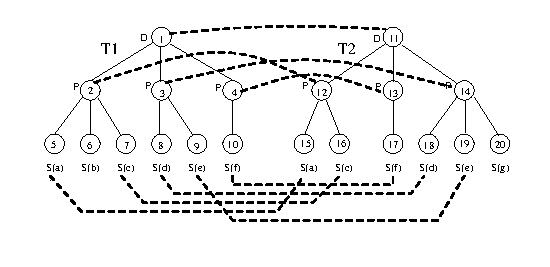
\includegraphics[width=\textwidth]
{../images/matching1.pdf}}
\caption{\label{fig:matching} Illustrates matching nodes in two revisions by dashes (from the paper "Change Detection in Hierarichally Structured
Data" by Chawathe \cite{chawathe1996change}).}
\end{figure}

\subsection{Tree-to-Tree Differences - Challenges}
In a nutshell the main challenges were the implementation of:

\begin{itemize}
\item Moves in Treetank with merging of adjacent text nodes.
\item A copy operation to insert whole subtrees (based on the visitor pattern).
\item One of the many existing ID-less algorithms (implemented the FMSE algorithm from Chawathe \cite{chawathe1996change}, whereas the algorithm in the paper seems to be inaccurate in two cases). The implementation is roughly based on the work of Daniel Hottinger and Franziska Meyer \cite{hottinger}, which have used DOM.
\item A LevelOrderAxis, which provides a breath first traversal to support the FSME algorithm.
\item An ID-based algorithm developed to compare revisions in Treetank.
\end{itemize}

Note that it is hard to track bugs in the FMSE algorithm since almost all code-units are dependent on each other.

\section{Future work}
Moves have recently been implemented in the backend (Treetank) to support FMSE and other ID-less difference algorithms which might be implemented in the future. To support moves in the visualizations the following three steps have to be implemented:

\begin{enumerate}
\item Optional support of moves in the ID-based algorithm.
\item Add \texttt{dummy}-nodes at the places where the nodes have been moved from (to speed up the algorithm which currently traverses the trees in a single preorder-traversal).
\item Splines to connect the dummy-nodes and moved nodes in the \emph{SunburstView}.
\end{enumerate}

Second the \emph{SmallMultiplesView} has to be synchronized with the \emph{SunburstView}. 

Furthermore to support sophisticated analytical tasks involving several revisions a specialized \texttt{XPathAxis} has to be implemented.

\bibliographystyle{abbrv}
\bibliography{bibtex}
\end{document}
